\SourcePage{GELFAND-P000452}{unlabelled}
\underline{\sout{\ldots}}.\qquad
\rule[.5ex]{13mm}{.35pt}\enspace$\cdot$\enspace\rule[.5ex]{17mm}{.35pt}
\Incomplete{GELFAND-P000452}{title-cancel}{Closely spaced wavy strokes cover the underlined heading. A stop is visible to the right. The letters are unresolved.}
\end{GelfandAdjacentEvidence}
\begin{GelfandAdjacentEvidence}{GELFAND-P000452}{2}


\underline{Manin’s 1st lecture on \mbox{$p$}-adic numbers.}\quad (retelling)

$K$ — loc. field, (\sout{\ldots}
\Incomplete{GELFAND-P000452}{k-cancel}{After the comma are a left parenthesis and a short, heavily cancelled inscription. The right parenthesis in this line is unclear.}
\end{GelfandAdjacentEvidence}
\begin{GelfandAdjacentEvidence}{GELFAND-P000452}{3}

(fin. ext. of the $p$-adic numbers)\quad
\sout{or form. pow. series over}\par\hspace{23mm}\sout{a fin. field})
\Incomplete{GELFAND-P000452}{parent-cancel-full}{The cancelled lines are provisionally read as “or form. pow. series over” and “a fin. field”. The closing parenthesis near “adic numbers” is heavily retraced.}
\end{GelfandAdjacentEvidence}
\begin{GelfandAdjacentEvidence}{GELFAND-P000452}{4}


\SourceFigure{GELFAND-P000452}{maximal-ideal-annotation}{A short vertical stroke connects $m$ with the label below.
\par\smallskip\centering\color{black}
\begingroup\color{black}\GelfandFitDiagram{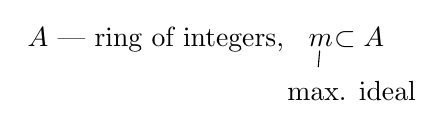
\begin{tikzpicture}[x=1mm,y=1mm,every node/.style={anchor=base west,inner sep=0pt}]
\node (ring) at (0,9) {$A$ — ring of integers,};
\node (ideal) at ([xshift=3mm]ring.base east) {$m$};
\node at (ideal.base east) {$\subset A$};
\draw ([xshift=-.15mm,yshift=-.4mm]ideal.south) -- ++(-.18,-2.1);
\node at ([xshift=-2.7mm,yshift=-6.8mm]ideal.base west) {max. ideal};
\end{tikzpicture}}\endgroup}
\end{GelfandAdjacentEvidence}
\begin{GelfandAdjacentEvidence}{GELFAND-P000452}{5}


$P^1(K)$ — proj. line.
\[
\begin{aligned}
G &= \text{its motions}\quad
   \left\{z\longrightarrow\frac{az+b}{cz+d}\ \middle|\ 
     a,b,c,d\in K,\ \det\ne0\right\}=\\
  &= \operatorname{GL}(2,K)/K^*
\end{aligned}
\]
\Unclear{GELFAND-P000452}{mobius-det}{The notation before the right brace reads $\det\ne0$. The sign is heavily retraced. Two horizontal strokes immediately after the brace read as $=$. The next line also starts with $=$.}
\end{GelfandAdjacentEvidence}
\begin{GelfandAdjacentEvidence}{GELFAND-P000452}{6}


$U\subset G$;\quad $U=\operatorname{GL}(2,A)/A^*$.

Constr. $G/U$ — graph $\Delta$ — analog of the Lobachevsky pl..

\underline{Def.}: a lattice in $K^2$ — a free $A$-module with 2 gen.
\[
L=Ae_1\oplus Ae_2.
\]
\underline{Lemma}. If $L_1$ and $L_2$ — 2 latt.,
then $\exists$ a basis $e_1,e_2$ in $K^2$, such that
\[
\begin{gathered}
L_1=Ae_1\oplus Ae_2;\qquad L_2=m^{\nu_1}e_1\oplus m^{\nu_2}e_2=\\
{}=A\pi^{\nu_1}e_1\oplus A\pi^{\nu_2}e_2
\end{gathered}
\]

\hfill($\pi$ — generator [?] of the max. ideal)
\Unclear{GELFAND-P000452}{ideal-symbol-tight}{A looped mark with a lengthwise stroke stands between “generator” and “max.” in the Russian. Its reading is unresolved.}
\end{GelfandAdjacentEvidence}
\begin{GelfandAdjacentEvidence}{GELFAND-P000452}{7}


\SourceFigure{GELFAND-P000452}{integer-note}{The inscription $\nu_1,\nu_2\in\mathbb Z$ sits at the right between the two parenthetical lines.
\par\smallskip\color{black}
(analog. to the lin. alg. theor. on simult. reduction)\hfill
\raisebox{1ex}{$\nu_1,\nu_2\in\mathbb Z$}}
\end{GelfandAdjacentEvidence}
\begin{GelfandAdjacentEvidence}{GELFAND-P000452}{8}


\underline{Def.}\quad $L_1\sim L_2$, if
\underline{$L_1=\alpha L_2$}, where $\alpha\in K^*$.

\begin{center}
\rule[.5ex]{17mm}{.35pt}\enspace$\cdot$\enspace\rule[.5ex]{19mm}{.35pt}
\end{center}
There is an analog of distance — as in symm. sp.. \sout{\ldots}\ — see \underline{A. Weil}
\Incomplete{GELFAND-P000452}{sim-margin-cancel}{The small sign before the dash is cancelled. Its reading is unresolved.}
\end{GelfandAdjacentEvidence}
\begin{GelfandAdjacentEvidence}{GELFAND-P000452}{9}


\begin{center}
\rule[.5ex]{17mm}{.35pt}\enspace$\cdot$\enspace\rule[.5ex]{19mm}{.35pt}
\end{center}
Vertices of graph $\Delta^{(0)}_{\text{\sout{\ldots}}}$ — equiv. classes of lattices
\Incomplete{GELFAND-P000452}{dimension-glyph}{A small cancelled sign appears below and to the right of the first $\Delta$. Its reading is unresolved. Above it is $(0)$.}
\end{GelfandAdjacentEvidence}


$G$ acts on $\Delta^{(0)}$.


\Needspace{7\baselineskip}
\begin{GelfandAdjacentEvidence}{GELFAND-P000453}{1}
